% \begin{savequote}[8cm]
% \textlatin{Cor animalium, fundamentum e\longs t vitæ, princeps omnium, Microco\longs mi Sol, a quo omnis vegetatio dependet, vigor omnis \& robur emanat.}

% The heart of animals is the foundation of their life, the sovereign of everything within them, the sun of their microcosm, that upon which all growth depends, from which all power proceeds.
%   \qauthor{--- William Harvey \cite{harvey_exercitatio_1628}}
% \end{savequote}

\chapter{\label{app:protocolmockup}Protocols and Mock-ups}

\minitoc

\section{Protocols}\label{app:protocol}
\subsection{Individual Interviews} 
For the individual interviews, we follow a semi-structured protocol, deviating when the conversation leads to interesting results related to our primary research questions:

\begin{enumerate}
    \item What is diveristy?
    \item Which elements of diversity matter in a talent identification context? Why?
    \item How would you envision technology assisting you in operationalising diversity?
\end{enumerate}

We interview 15 individuals from two different talent identification organisations. We conduct each interview separately. We first ask a few questions about the factors that go into decision-making.

\begin{enumerate}
    \item We're going to take a step back and discuss a hypothetical selection scenario for a fellowship for a group of young people. In this scenario, you have full control over who is selected.
    \item Could you please list some things you think are important in deciding who to accept?
    \item (Can skip) Which of (these things) are about the individual applicant's performance?
    \item What are (these remaining things) about? 
    \item (Or:) Why are (these things) important?
\end{enumerate}

We then ask participants to define diversity, to break it down into elements, and to discuss why diversity is important.

\begin{enumerate}
    \item Now I want to talk about diversity. Keeping your list in mind, can you please define diversity?
    \item (If the definition is too short) Could you please elaborate on (pick a part)
    \item Why do we care about this definition of diversity?
    \item Now, if you were going to break your definition into some elements or facets, what would those be?
    \item (If they talk about holistic diversity) What considerations are important when looking at diversity holistically?
    \item (If elements are vague) How does (pick a metric) factor into your understanding of (element)?
    \item Which elements or considerations are most important?
    \item How do we measure these facets of diversity?
    \item (If this measurement isn't concrete) Imagine you had a “magic metric” that perfectly measured diversity. What does this metric do?
\end{enumerate}

Next, we run two short exercises from the participatory design literature. The first is called ``crazy 8s'', wherein participants are given 8 minutes to come up with 8 ideas. For these ideas, we ask participants to think about technologies that might help them better understand diversity in selection.

\begin{enumerate}
    \item Now I want to talk about technology we can build to support thinking about tradeoffs around diversity. Remember that we're stepping away from existing processes and solutions.
    \item We're going to start with an exercise called “crazy 8s”. For the next 8 minutes, we're going to spend one minute each developing a technology that might help us better understand diversity in selection. These technologies don't have to make sense or be possible; I just want you to think of things that might help you think through diversity. This activity is difficult; don't worry if you find yourself struggling or sounding silly.
    \item Take a second to think about a technology. When you're ready, please describe it.
    \item (If the technology is unclear) Could you please elaborate on (unclear part)?
\end{enumerate}

The second is called ``the magic app'', wherein participants are asked to elaborate on a single idea for an application, waving away technical details as `magic'.

\begin{enumerate}
    \item Now let's dig deeper into one hypothetical “magic app” designed to help us better understand tradeoffs around diversity in selection. The magic app can do anything you might want it to in any way you might want. What does your magic app do?
    \item (If the app has visuals) What do your visuals look like?
    \item (If the app is pure text) What sorts of visualisations might help you?
    \item (If the app has buttons or sliders) What do your buttons do?
    \item (If the app doesn't have any interactivity) How might you interact with this app?
    \item Now we are going to split the app out into different “pages”
    \item (If they haven't already done this) The individual-level page: each applicant will have their own individual-level page, which will say things about that applicant
    \item (If they haven't already done this) The cohort-level page: each possible cohort will have its own cohort-level page, which will update any time we make changes to the cohort.
    \item (For each page) What happens on this page?
    \item What is the experience of using this page like?
    \item (If the page has visuals) What do your visuals look like?
    \item (If the page is pure text) What sorts of visualisations might help you?
    \item (If the page has buttons or sliders) What do your buttons do?
    \item (If the page doesn't have any interactivity) How might you interact with this app?
    \item (For each different feature of the page) What makes (feature) useful to you?
    \item Thank you! Is there anything else you would like to add?
\end{enumerate}

\subsection{Design Workshops}
For the participatory design workshops, we split our participants by organization. As some individuals could not attend the second session, we have one group of 6 and another of 7. As these are much larger group discussions, we deviate further from our protocol.

The task for these workshops consists of hands-on sessions with different technologies. The technologies are designed and mocked up based on the thematic analysis of the interviews. These technologies are presented to participants via Miro, where they are free to interact with and annotate them. Our research question for this workshop is, for each mock-up: ``How can this mock-up help you better promote diversity in talent identification?''.

For each technology mock-up shown, we ask the following questions:

\begin{enumerate}
    \item This mock-up describes... Are any of you familiar with this?
    \item In what follows, we're going to discuss this mock-up. Let's start with: is it easy to read for you? What does it say? 
    \item What questions do you have upon seeing this mock-up? Feel free to write these down.
    \item How would you use this mock-up in a hypothetical selection procedure?
    \item How (else) would this mock-up fit into your current selection procedure?
    \item How would your current selection procedure make best use of this mock-up? Would the process need to be changed? Do you think this would be beneficial?
\end{enumerate}

Finally, at the end of our workshop, after we have covered all of the mock-ups, we ask participants to place a star next to their favourite mock-up on the Miro board.

\section{Mock-ups}\label{app:mockups}
Here we present the six mock-ups we used in our design workshops. Three of these mock-ups (Figures \ref{fig:representativeness}, \ref{fig:entropy}, and \ref{fig:diversity}) present information about the range of possible cohorts participants must choose between, while three of these mock-ups (Figures \ref{fig:demographic}, \ref{fig:impact}, and \ref{fig:advantage}) present information about an individual applicant relative to a given cohort and a given pool.

\begin{figure}[htbp]
    \centering
    \begin{subfigure}[b]{0.3\textwidth}
        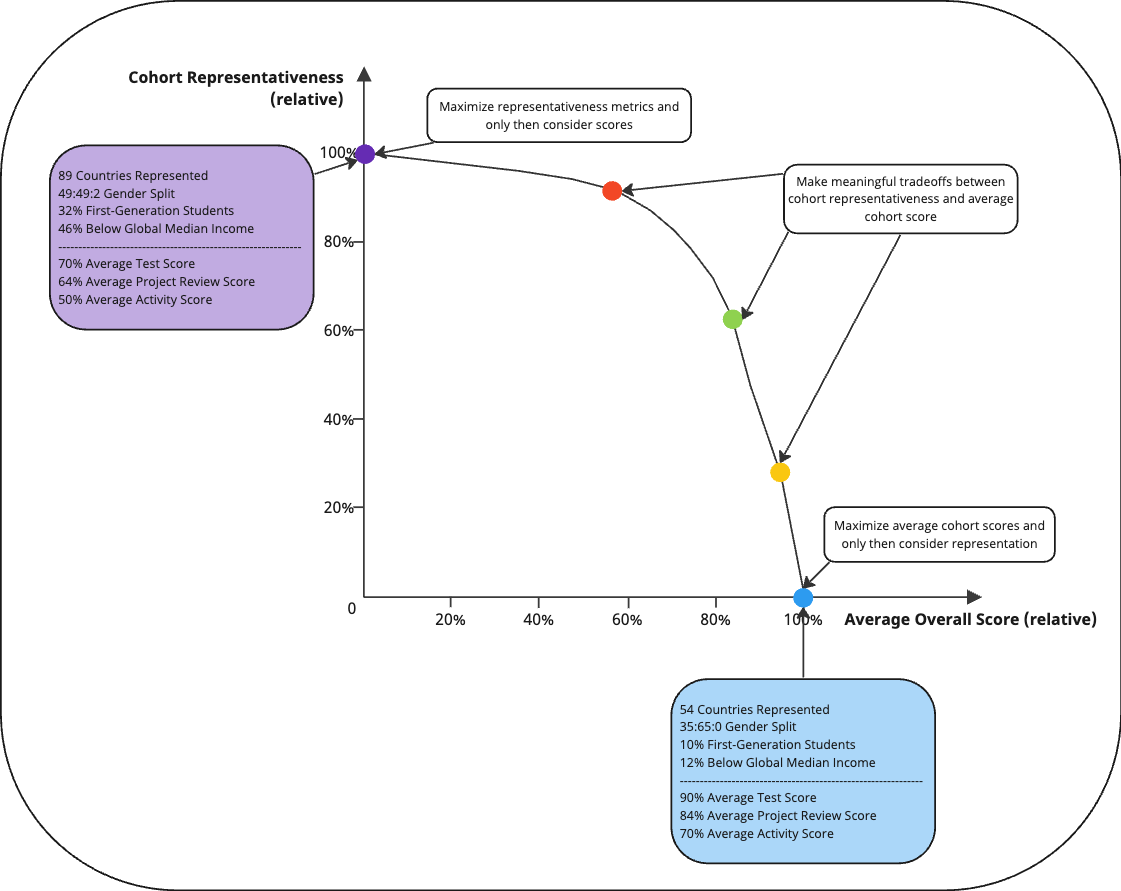
\includegraphics[width=\textwidth]{figures/representativeness.png}
        \caption{Mock-up 1: Cohort Representativeness}
        \label{fig:representativeness}
    \end{subfigure}
    \hfill
    \begin{subfigure}[b]{0.3\textwidth}
        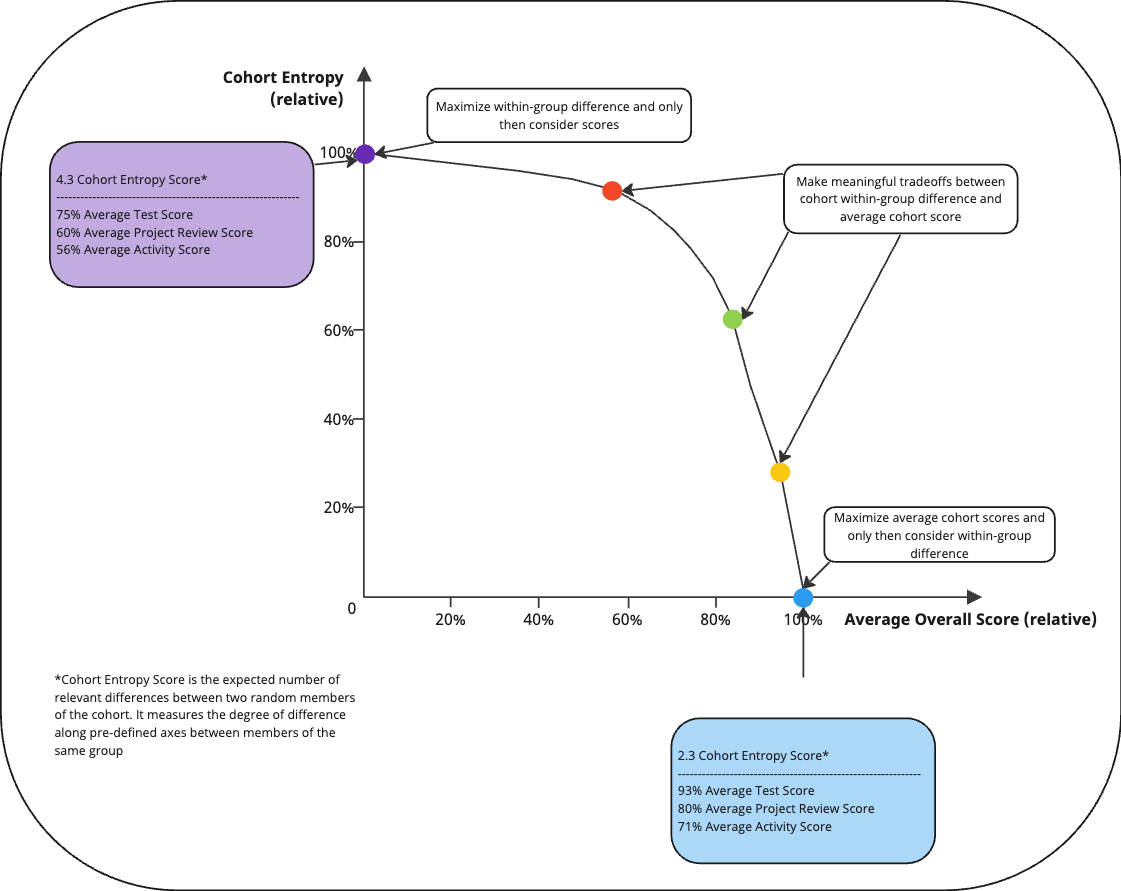
\includegraphics[width=\textwidth]{figures/entropy.png}
        \caption{Mock-up 2: Cohort Entropy}
        \label{fig:entropy}
    \end{subfigure}
    \hfill
    \begin{subfigure}[b]{0.3\textwidth}
        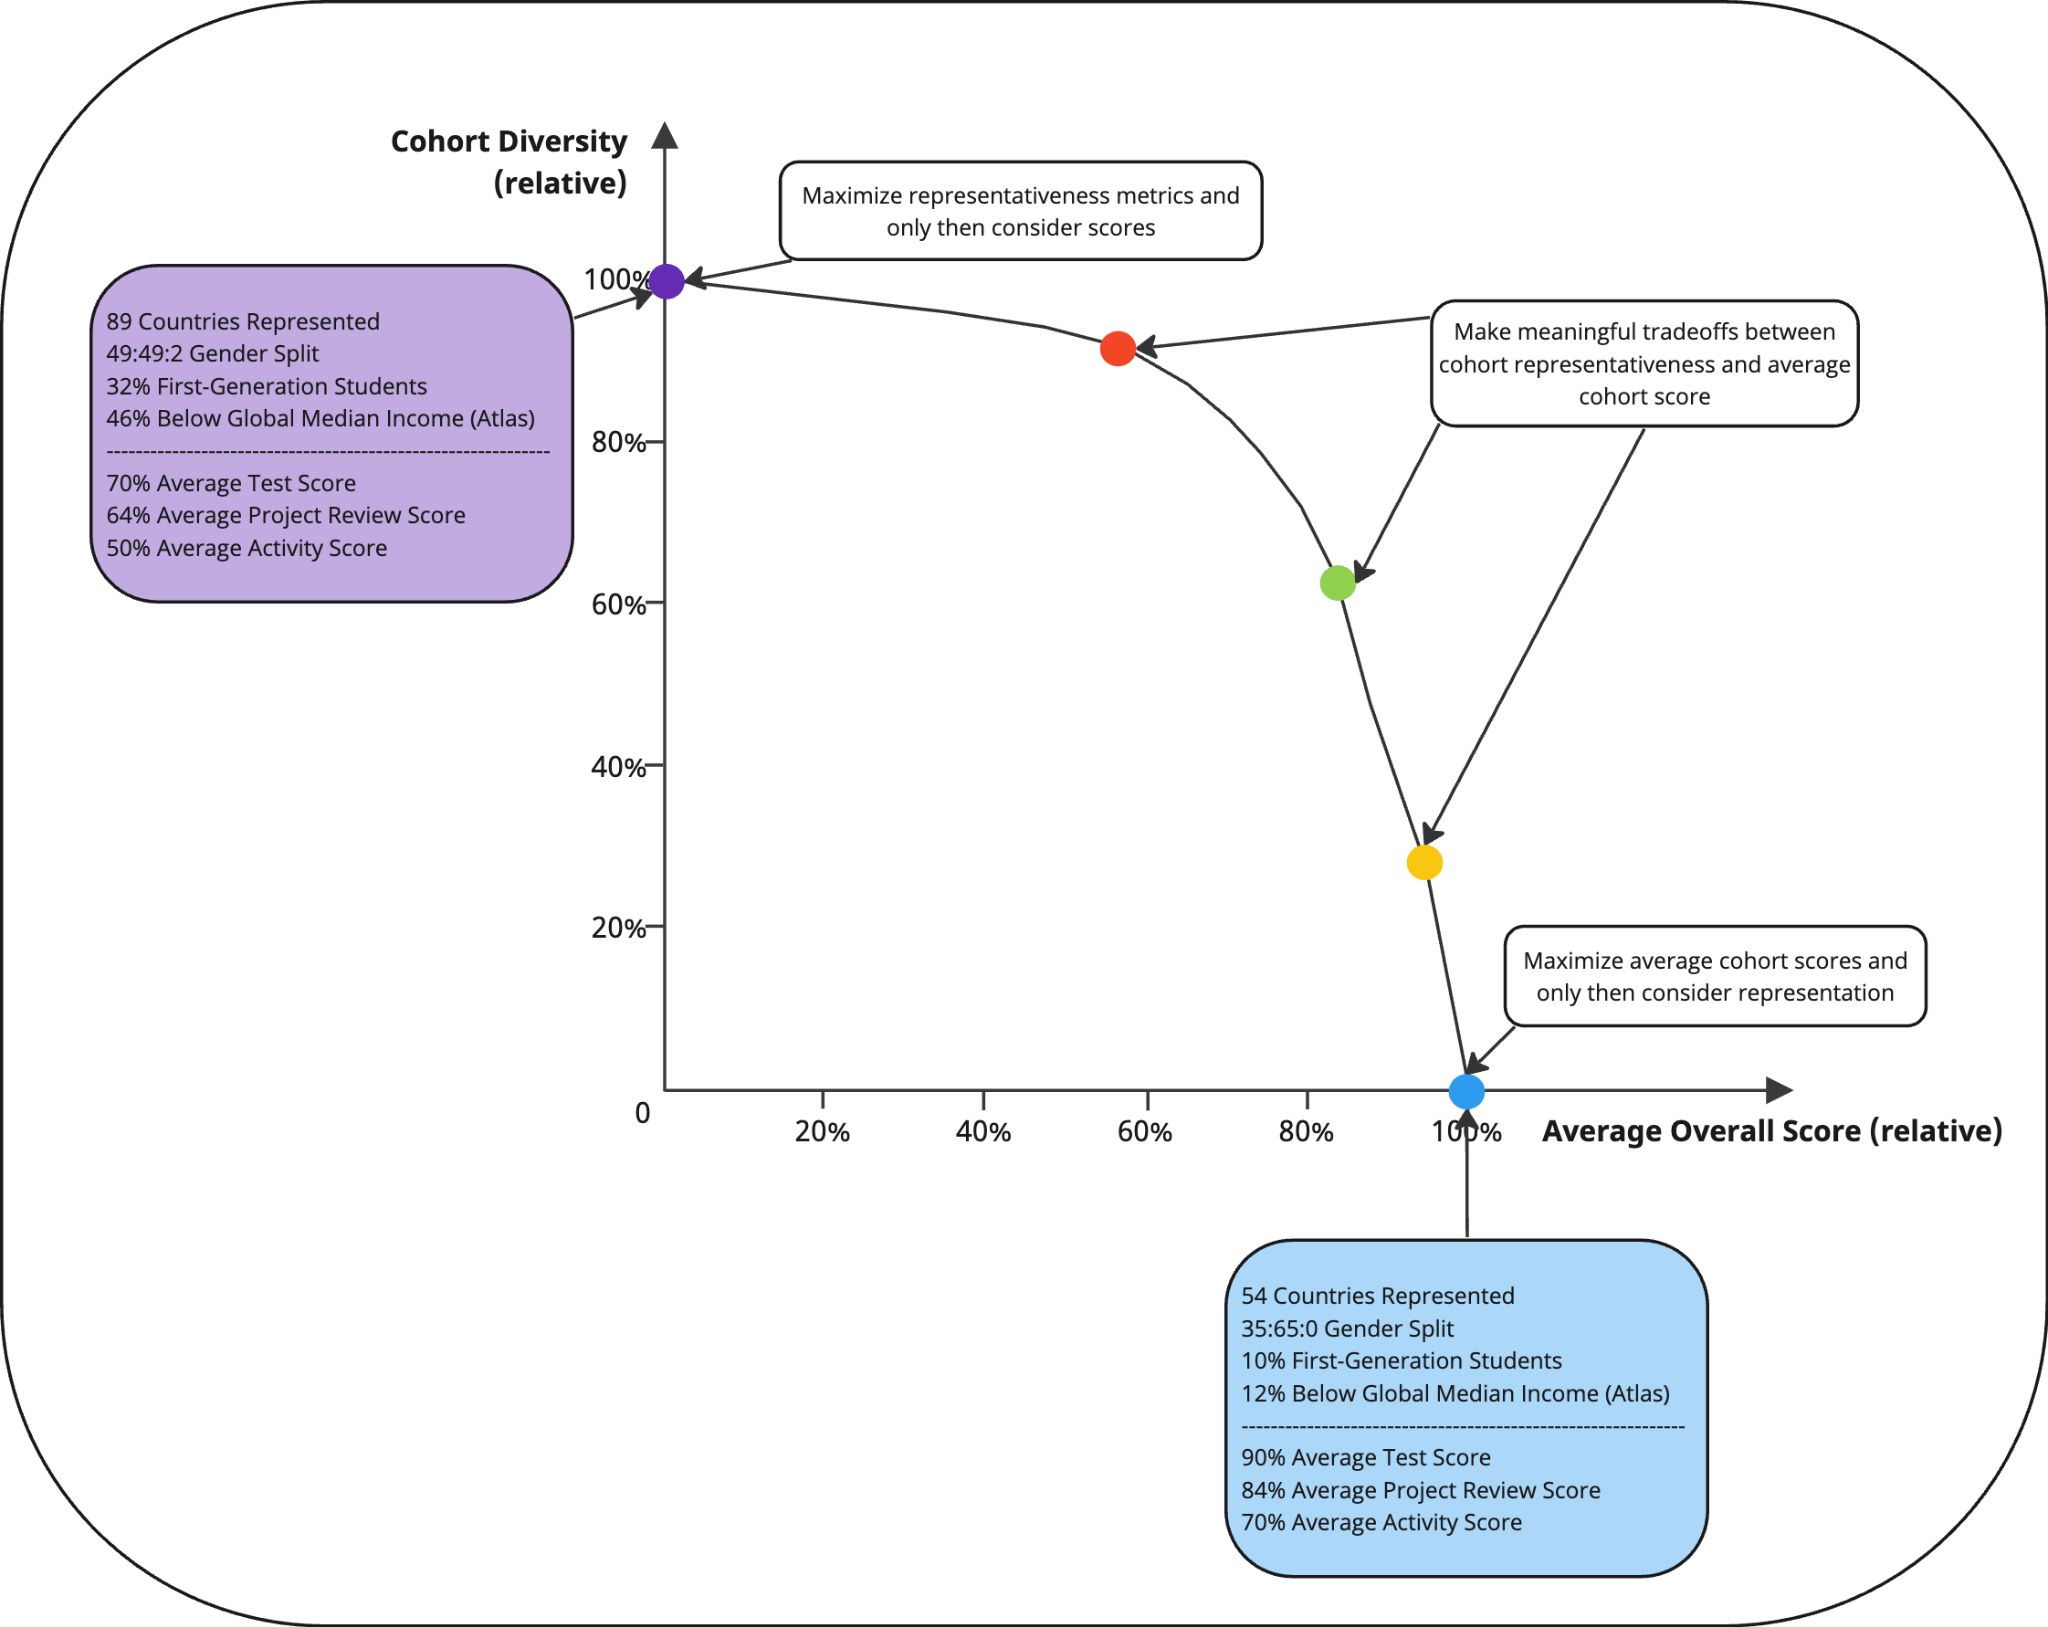
\includegraphics[width=\textwidth]{figures/diversity.png}
        \caption{Mock-up 3: Cohort Diversity}
        \label{fig:diversity}
    \end{subfigure}

    \medskip

    \begin{subfigure}[b]{0.3\textwidth}
        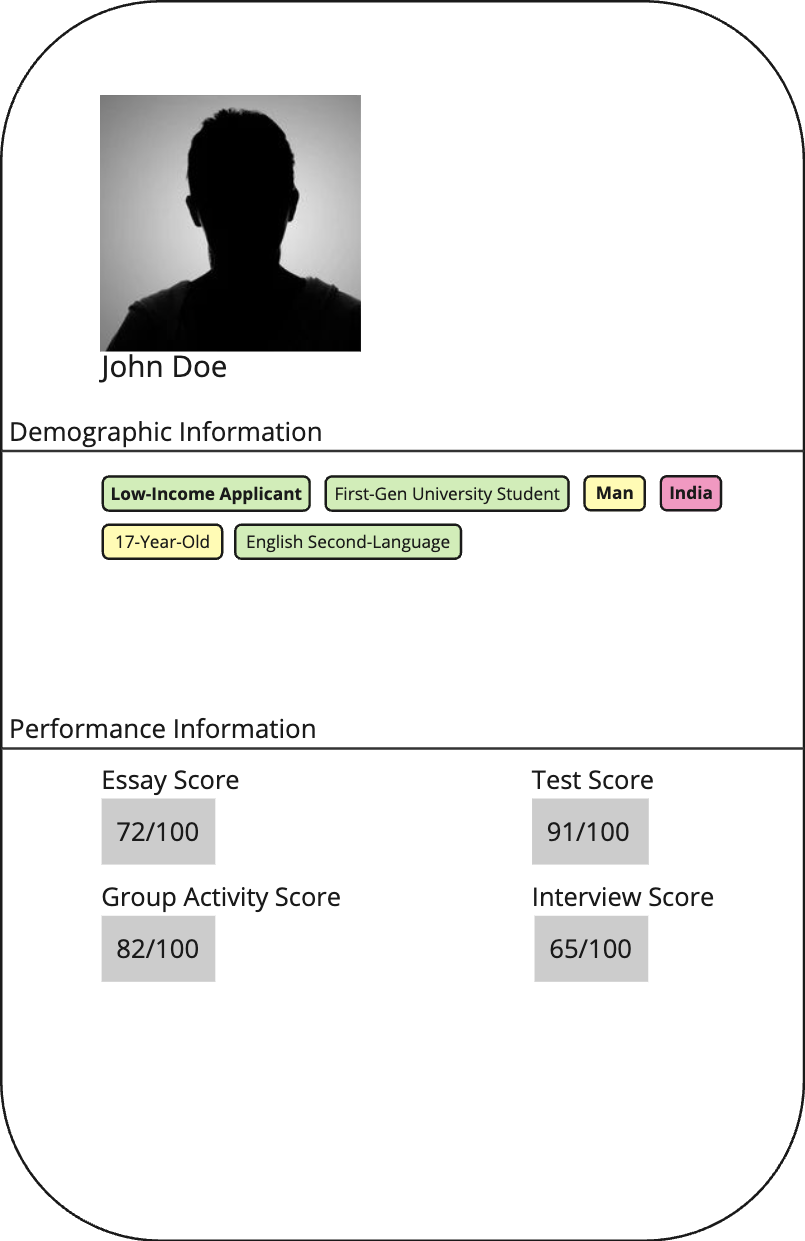
\includegraphics[width=\textwidth]{figures/demographic.png}
        \caption{Mock-up 4: Applicant Demographic Information}
        \label{fig:demographic}
    \end{subfigure}
    \hfill
    \begin{subfigure}[b]{0.3\textwidth}
        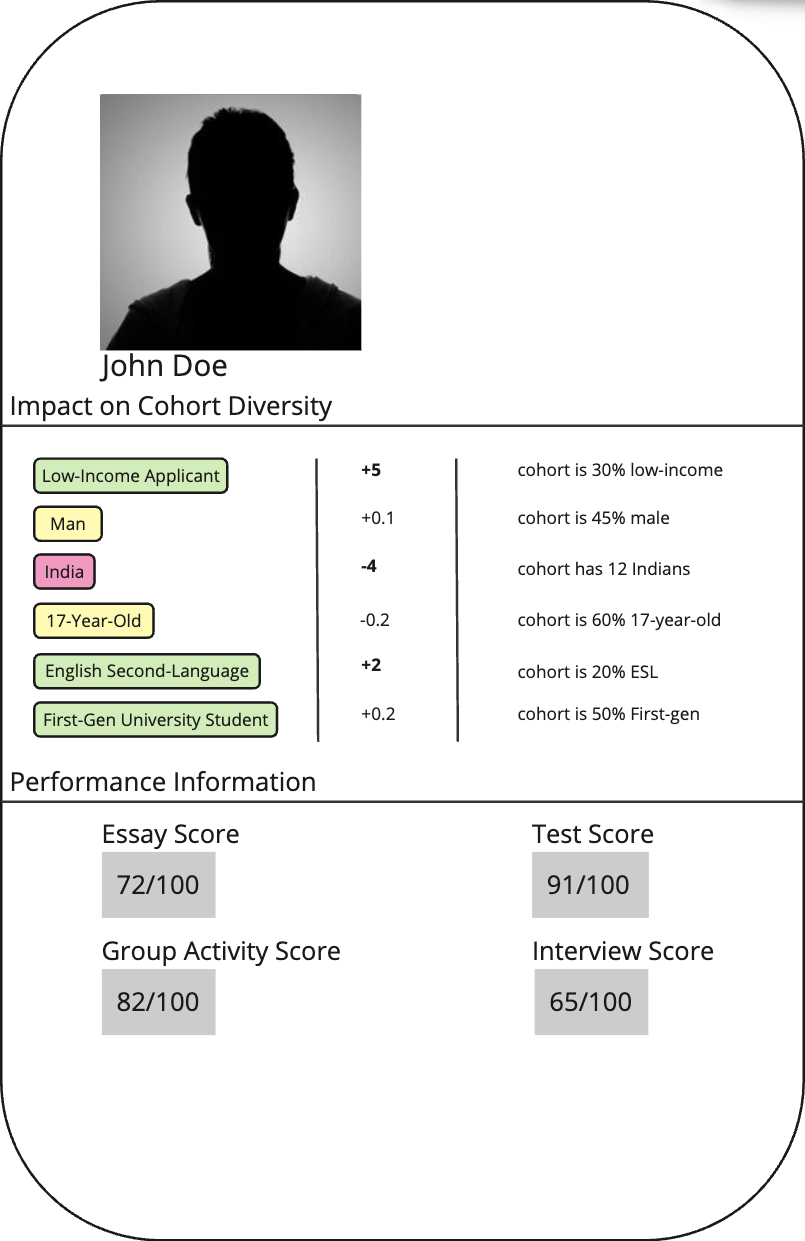
\includegraphics[width=\textwidth]{figures/impact.png}
        \caption{Mock-up 5: Applicant Demographic Impact on Cohort}
        \label{fig:impact}
    \end{subfigure}
    \hfill
    \begin{subfigure}[b]{0.3\textwidth}
        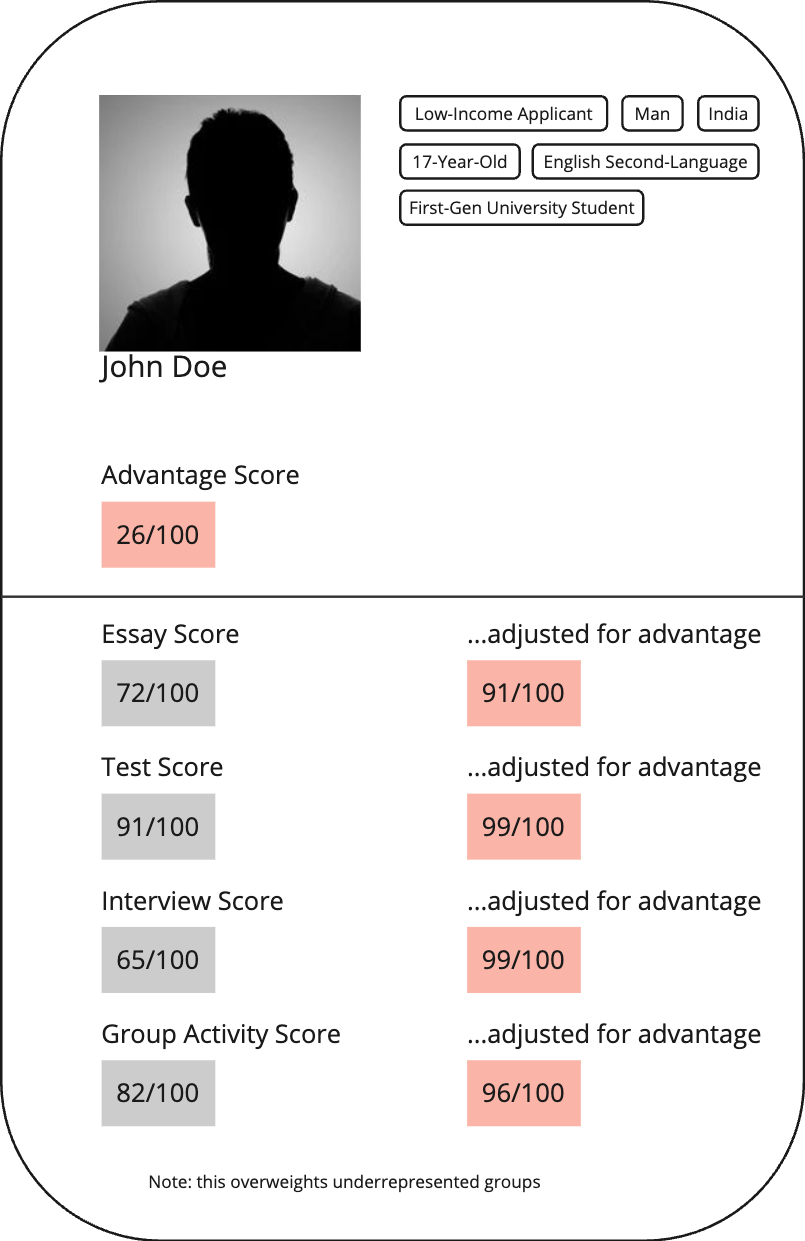
\includegraphics[width=\textwidth]{figures/advantage.png}
        \caption{Mock-up 6: Applicant Advantage Scores}
        \label{fig:advantage}
    \end{subfigure}
    \caption{Main caption for the figure}
    \label{fig:mockups}
\end{figure}